\documentclass[showpacs,preprintnumbers,amsmath,amssymb,superscriptaddress,aip]{revtex4-1}
\usepackage{graphicx}
%\setlength{\parindent}{0in}

% General Latex  --------------------------------------------------
\def\beq{\begin{equation}}
\def\eeq{\end{equation}}
\def\beqar{\begin{eqnarray}}
\def\eeqar{\end{eqnarray}}
\def\nn{\nonumber}
\def\ol{\overline}
\def\para{\parallel}

% Operators  ------------------------------------------------------
\newcommand{\diff}[2]{\frac{d#1}{d#2}}
\newcommand{\diffs}[2]{\frac{d^2#1}{d#2^2}}
\newcommand{\pdiff}[2]{\frac{\partial#1}{\partial#2}}
\newcommand{\pdiffs}[2]{\frac{\partial^2#1}{\partial#2^2}}
\newcommand{\pdiffxy}[3]{\frac{\partial^2#1}{\partial#2 \partial#3}}
\newcommand{\pdt}{\partial_t}
\newcommand{\pdr}{\partial_r}
\newcommand{\pdth}{\partial_\theta}
\newcommand{\pdrr}{\partial^2_r}

\newcommand{\enum}[2]{{#1}\times10^{#2}} % 4.2x10^{3} = \enum{4.2}{3}

\newcommand{\vect}[1]{{\bf #1}}
%\newcommand{\vect}{\overrightarrow}
%\newcommand{\vect}{\vec}
\def\div{\nabla\cdot}
\def\grad{\nabla}
\def\curl{\nabla\times}
\newcommand{\gradpar}{\grad_\parallel}
\newcommand{\gradperp}{\grad_\perp}
\newcommand{\gradr}{\grad_r}
\newcommand{\defeq}{\ensuremath{\stackrel{\text{\tiny def}}{=}}}

\newcommand{\savg}[1]{\left<{#1}\right>}
\newcommand{\vavg}[1]{\left<{#1}\right>_V}
\newcommand{\thavg}[1]{\left<{#1}\right>_\theta}

% Variable names  -------------------------------------------------
\newcommand{\vpar} {v_\parallel}
\newcommand{\Apar} {A_\parallel}
\newcommand{\jpar} {j_\parallel}
\newcommand{\kpar} {k_\parallel}
\newcommand{\kperp} {k_\perp }
\newcommand{\vperp} {v_\perp }
\newcommand{\kthe}{k_\theta}

\newcommand{\Evec}{\ensuremath{\boldsymbol{{\rm E}}}}
\newcommand{\Bvec}{\ensuremath{\boldsymbol{{\rm B}}}}
\newcommand{\Jvec}{\ensuremath{\boldsymbol{{\rm J}}}}
\newcommand{\Fvec}{\ensuremath{\boldsymbol{{\rm F}}}}
\newcommand{\fvec}{\ensuremath{\boldsymbol{{\rm f}}}}
\newcommand{\vE}{\ensuremath{\boldsymbol{{\rm v}_{E}}}}
\newcommand{\bo}{\ensuremath{\boldsymbol{{\rm b}_0}}}
\newcommand{\bvec}{\ensuremath{\boldsymbol{{\rm b}}}}
\newcommand{\xvec}{\ensuremath{\boldsymbol{{\rm x}}}}
\newcommand{\yvec}{\ensuremath{\boldsymbol{{\rm y}}}}
\newcommand{\zvec}{\ensuremath{\boldsymbol{{\rm z}}}}
\newcommand{\vvec}{\ensuremath{\boldsymbol{{\rm v}}}}
\newcommand{\jvec}{\ensuremath{\boldsymbol{{\rm j}}}}

\newcommand{\bxgp}{\bvec\times\gradperp}

\newcommand{\vve}{\ensuremath{\boldsymbol{{\rm v}}_{e}}}
\newcommand{\vvi}{\ensuremath{\boldsymbol{{\rm v}}_{i}}}
\newcommand{\vpe}{v_{\parallel e}}
\newcommand{\vpi}{v_{\parallel i}}
\newcommand{\vvE}{\ensuremath{\boldsymbol{{\rm v}}_{E}}}
\newcommand{\vvD}{\ensuremath{\boldsymbol{{\rm v}}_{D}}}

\newcommand{\nuei}{\nu_{ei}}
\newcommand{\nuii}{\nu_{ii}}
\newcommand{\nue}{\nu_{e}}
\newcommand{\nuen}{\nu_{en}}
\newcommand{\nuin}{\nu_{in}}
\newcommand{\kpe}{\kappa_{\parallel e}}

\newcommand{\rs}{\rho_{s}}
\newcommand{\ri}{\rho_{i}}
\newcommand{\wci}{\Omega_{i}}
\newcommand{\wcix}{\Omega_{ix}}
\newcommand{\wce}{\Omega_{e}}
\newcommand{\tomega}{\tilde\omega}
\newcommand{\Isat}{I_{\rm sat}}
\newcommand{\fmie}{\frac{m_i}{m_e}}
\newcommand{\fmei}{\frac{m_e}{m_i}}


% Often used dimensions
\newcommand{\cm}{\rm cm}
\newcommand{\mm}{\rm mm}
\newcommand{\cmn}{{\rm cm}^{-3}}
\newcommand{\mn}{{\rm m}^{-3}}
\newcommand{\eV}{\rm eV}
\newcommand{\G}{\rm G}
\newcommand{\T}{\rm T}



\begin{document}

\title{Energy dynamics in a simulation of LAPD turbulence}

\author{B. Friedman}
\email{friedman@physics.ucla.edu}

\author{T.A. Carter}

\affiliation{Department of Physics and Astronomy, University of California, Los Angeles, California 90095-1547, USA}

\author{M.V. Umansky}
\affiliation{Lawrence Livermore National Laboratory, Livermore, California 94550, USA}

\author{D. Schaffner}

\affiliation{Department of Physics and Astronomy, University of California, Los Angeles, California 90095-1547, USA}

\author{I. Joseph}

\affiliation{Lawrence Livermore National Laboratory, Livermore, California 94550, USA}




\begin{abstract}
Abstract
\end{abstract}

\maketitle

\section{Introduction}


\section{The drift wave model}
\label{dw_model}

A Braginskii-based fluid model~\cite{Braginskii1965} is used to simulate drift wave turbulence in LAPD using the BOUT++ code~\cite{dudson2009}. 
The evolved variables in the model are the plasma density, $N$, the electron fluid parallel velocity $\vpe$, the potential vorticity $\varpi \equiv \gradperp \cdot (N_0 \gradperp \phi)$,
and the electron temperature $T_e$. The ions are assumed cold in the
model ($T_i = 0$), which eliminates ion temperature gradient drive,
and sound wave effects are neglected. Details of the simulation code, derivations of the model, grid convergence studies, and analyses of simplified models
may be found in previous LAPD simulation studies~\cite{Popovich2010a,Popovich2010b,Umansky2011,friedman2012,friedman2012b}.

The equations are developed with Bohm normalizations: lengths are
normalized to the ion sound gyroradius, times to the ion
cyclotron time, velocities to the sound speed, densities to the equilibrium peak density, and electron
temperatures and potentials to the equilibrium peak electron temperature. These normalizations are constants (not functions of radius) and are calculated from these reference values:
the magnetic field is $1$ kG, the ion unit mass is $4$, the peak density is $2.86 \times 10^{12}$ cm$^{-3}$, and the peak electron temperature
is $6$ eV. The equations are:

\beqar
\label{ni_eq}
\pdt N = - {\mathbf v_E} \cdot \grad N_0 - N_0 \gradpar \vpe + \mu_N \gradperp^2 N + S_N + \{\phi,N\}, \\
\label{ve_eq}
\pdt \vpe = - \fmie \frac{T_{e0}}{N_0} \gradpar N - 1.71 \fmie \gradpar T_e  + \fmie \gradpar \phi - \nue \vpe + \{\phi,\vpe \}, \\
\label{rho_eq}
\pdt \varpi = - N_0 \gradpar \vpe  - \nuin \varpi + \mu_\phi \gradperp^2 \varpi + \{\phi,\varpi \}, \\
\label{te_eq}
\pdt T_e = - {\mathbf v_E} \cdot \grad T_{e0} - 1.71 \frac{2}{3} T_{e0} \gradpar \vpe + \frac{2}{3 N_0} \kpe \gradpar^2 T_e  \nonumber \\
- \frac{2 m_e}{m_i} \nue T_e  + \mu_T \gradperp^2 T_e +  S_T + \{\phi,T_e\}.
\eeqar

In these equations, $\mu_N$, $\mu_T$, and $\mu_\phi$ are artificial diffusion and viscosity coefficients used for subgrid dissipation. They are large enough to allow saturation
and grid convergence~\cite{friedman2012}, but small enough to allow for turbulence to develop. In the simulations, they are all given the same value of $1.25 \times 10^{-3}$ in Bohm-normalized units. 
This is the only free parameter in the simulations. All other parameters such as the electron collisionality $\nue$, ion-neutral
collisionality $\nuin$, parallel electron thermal conductivity $\kpe$, and mass ratio $\fmie$ are calculated from the experimental parameters.
There are two sources of free energy: the density gradient due to the equilibrium density profile $N_0$, and the equilibrium electron temperature gradient in $T_{e0}$, both of which are
taken from experimental fits. $N_0$ and $T_{e0}$ are functions of only the radial cylindrical coordinate $r$, and they are shown in Fig.~\ref{eq_profiles}. The simulations are therefore global.

Simulations also use density and temperature sources ($S_n$ and $S_T$) in order to keep the equilibrium profiles from relaxing away from their experimental shapes. 
These sources suppress the azimuthal averages ($m=0$ component of the density and temperature fluctuations) at each time step. 
The azimuthal average of the potential $\phi$ is allowed to evolve in
the simulation, allowing zonal flows to arise.

The terms in Poisson brackets are the $E \times B$ advective nonlinearities, which are the only nonlinearities used in the simulations.
The numerical simulations are fully spatial in all three dimensions (as opposed to spectral) and use cylindrical annular geometry ($12<r<40$ cm). The radial extent used in the simulation
encompasses the region where fluctuations are above a few percent in the experiment. Therefore, the radial boundaries are fixed to zero value.

This study analyzes three turbulent simulations which will be referred to as the periodic simulation, the no $n=0$ simulation, and the sheath simulation.
The periodic and no $n=0$ simulations were also analyzed in a previous paper~\cite{friedman2012b}. Both of these simulations enforce periodic boundary conditions in the axial ($z$)
direction (hence the label periodic). The no $n=0$ simulation adds an artificial sink-like contribution to Eqns.~\ref{ni_eq}-\ref{te_eq} which removes the axial average 
($k_\parallel = n = 0$ contribution) of the fluctuations at each time step. The previous study showed that this no $n=0$ essentially eliminated nonlinear instability drive and allowed
the linear instability to take over the turbulent drive.

Now the third (sheath) simulation is new. 
All previous LAPD simulation studies by this group used periodic axial boundary conditions~\cite{Popovich2010a,Popovich2010b,Umansky2011,friedman2012,friedman2012b}.
The sheath simulation, as its name implies, uses sheath boundary conditions on the axial machine ends. Specifically, the sheath boundary
condition for the parallel current is a linearized Bohm condition:

\beq
\label{sheath_bndry}
J_\para = N_0 (\phi + \text{log} \sqrt{4 \pi m_e/m_i} \ T_e) 
\eeq

where $J_\para = - N_0 \vpe$. The axial boundaries for the other independent fields are implemented with zero derivative (Neumann) boundary conditions, which is consistent with
analytical and numerical calculations for such fields in the magnetic pre-sheath region~\cite{loizu2012}. 
This study will in part compare results from the three simulations to help illustrate any effects of the sheath boundary conditions.

As a first comparison, Fig.~\ref{statistics} shows a few statistical characteristics of the density fluctuations for each of the three simulations along with the corresponding
characteristics from the experiment. The periodic simulation clearly has the most similar characteristics to those of the experiment while the no $n=0$ simulation is most dissimilar.
The fluctuations of the sheath simulation do have quite similar statistical properties to the experiment, however, the amplitude of the sheath simulation fluctuations is a bit smaller
than the experimental fluctuations, especially at small radii.

\begin{figure}[!htbp]
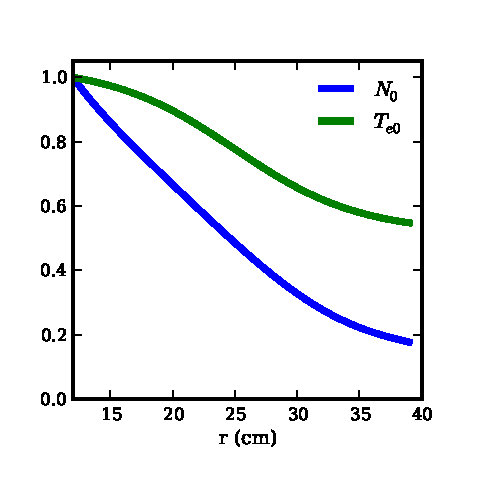
\includegraphics[]{equilibrium_profiles}
\hfil
\caption{The profiles of density $N_0$ and electron temperature $T_{e0}$ used in the simulations normalized to their peak values of $2.86 \times 10^{12}$ cm$^{-3}$ and 
$6$ eV, respectively.}
\label{eq_profiles}
\end{figure}

\begin{figure}[!htbp]
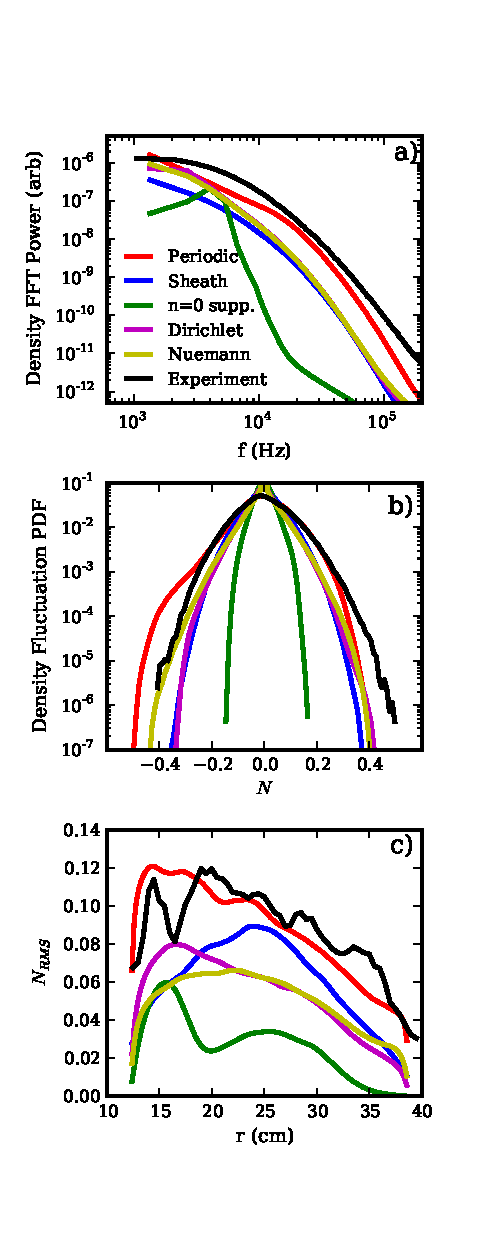
\includegraphics[]{statistics}
\hfil
\caption{A comparison of the statistical turbulent properties of the density field. The figures show \textbf{a)} the frequency spectrum, \textbf{b)} the pdf and \textbf{c)} the RMS level
of the fluctuations as a function of radius. The various curves use data calculated from the experiment, the simulation with periodic boundary conditions, the simulation with sheath
boundary conditions, and a simulation where the $n=0$ components of the fluctuations are artificially removed.}
\label{statistics}
\end{figure}


\section{Linear Instabilities}
\label{sec_linear}

\begin{figure}[!htbp]
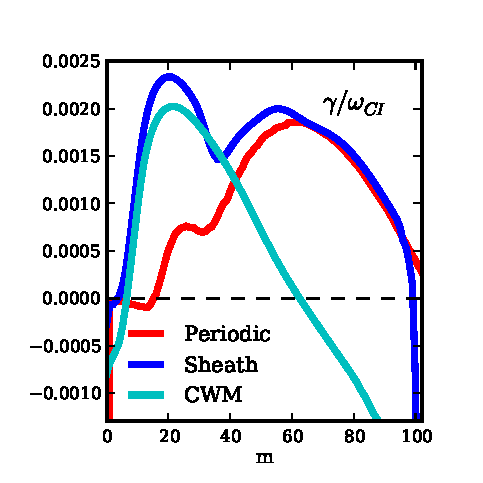
\includegraphics[width=0.6\textwidth]{gamma_comparisons}
\hfil
\caption{The growth rates of the drift waves, the conducting wall mode, and the full combined model.}
\label{drift_cwm_gamma}
\end{figure}


The model described by the equations of Section~\ref{dw_model} contains a few linear instabilities that can all act at the simulated scales. Two of these instabilities are of the electrostatic
drift wave type - one is driven by the density gradient and the other by the electron temperature gradient. Both of these instabilities gain access to the electrostatic potential through parallel
compression, called the adiabatic response, and are made unstable by the electron-ion collisional dissipation. These instabilities act under either choice of parallel boundary conditions 
(periodic or sheath).

The other instability is called the conducting wall mode (CWM) since it is driven by the conducting wall sheaths on the parallel boundaries. Eqs.~\ref{ni_eq}-\ref{te_eq} can be reduced to a smaller
set to isolate the conducting wall mode. The reduced set of linearized equations are:

\beqar
\label{ve_eq2}
\pdt \vpe = \fmie \gradpar \phi - \nue \vpe, \\
\label{rho_eq2}
\pdt \varpi = - N_0 \gradpar \vpe - \nuin \varpi + \mu_\phi \gradperp^2 \varpi, \\
\label{te_eq2}
\pdt T_e = - {\mathbf v_E} \cdot \grad T_{e0} + \frac{2}{3 N_0} \kpe \gradpar^2 T_e  - \frac{2 m_e}{m_i} \nue T_e  + \mu_T \gradperp^2 T_e,
\eeqar

along with the axial boundary condition given in Eq.~\ref{sheath_bndry}. The free energy source for this instability is the electron temperature gradient, which is also the free energy
for the thermally driven drift waves. However, the adiabatic response is replaced here with a coupling to the potential through the axial boundary condition.

Now, for the experimental parameters and profiles used in the simulations, 
the growth rates for the drift waves and the conducting wall mode are comparable. The fastest growth rates as a function of azimuthal wavenumber
are shown in Fig.~\ref{drift_cwm_gamma}.
The drift wave growth rate curve is found by simulating the linearized versions of Eqs.~\ref{ni_eq}-\ref{te_eq} with periodic axial boundary conditions in BOUT++. Therefore, both the density- and
temperature-drive drift wave contributions are combined in obtaining these growth rates. This is the linearized version of the model used in the previous study~\cite{friedman2012b}.
The CWM curve is obtained by simulating Eqs.~\ref{ve_eq2}-\ref{te_eq2} with the sheath axial boundary condition of Eq.~\ref{sheath_bndry}. 
Finally, the sheath model curve includes all of Eqs.~\ref{ni_eq}-\ref{te_eq} along with the axial sheath boundary condition.


\section{Energetics Machinery}
\label{sec_energetics_machinery}

In order to perform an energy dynamics analysis on the simulations, expressions for the energy and energy evolution must be derived from Eqs.~\ref{ni_eq}-\ref{te_eq}.
To start, an expression for the normalized energy of the wave fluctuations in the drift wave model is defined as:

\beq
\label{energy_eq}
E = \frac{1}{2} \int_V  \left[ P_0 \left((N/N_0)^2 + \frac{3}{2} (T_e/T_{e0})^2 \right) + N_0 \left( \frac{m_e}{m_i} \vpe^2 + (\gradperp \phi)^2 \right) \right] dV,
\eeq

where $P_0 = N_0 T_{e0}$ is the equilibrium pressure.
The $N^2$ contribution is the potential energy due to density fluctuations, $T_e^2$ is the electron temperature fluctuation potential energy,
$\vpe^2$ is the parallel electron kinetic energy, and $(\gradperp \phi)^2$ is the $E \times B$ perpendicular kinetic energy.
This energy expression is the physical fluctuation energy. This expression differs slightly from the energy-like expression used in the previous work~\cite{friedman2012b} in that it contains
extra factors of $N_0$ and $T_{e0}$. The energy-like expression that was analyzed in the previous work was chosen because it had the convenient property that it conserved the advective nonlinearities.
The advective nonlinearities are not conserved under the physical energy as defined in Eq.~\ref{energy_eq}, but the advective nonlinearities are also not conserved when the boundaries are not
periodic or fixed valued. Since the sheath boundary conditions used here do not have this feature, the advective nonlinearities would not be conserved under any general energy expression in any case.
So there is no similar advantage in this case to using a special energy-like expression. It is actually more convenient to use the physical energy rather than the special form used in the 
previous work for a different reason. 
The reason is that the physical energy conserves the parallel compression dynamics, which means that net energy cannot enter directly into
the parallel kinetic energy channel but must make its way via the density or temperature potential energy, which is physically meaningful and simpler to analyze. 
Now, while the energy-like expression used in the previous work did not preserve this property, the energy that directly entered the parallel kinetic energy channel was too small to matter 
qualitatively~\cite{friedman2012b}.

A more detailed look at the energetic processes comes from a spectral energy analysis. To do this, each fluid field $(N,T_e,\vpe,\phi)$ at a given time is Fourier decomposed as 
$F(r,\theta,z) = \sum_{\vec{k}} f_{\vec{k}}(r) e^{i (m \theta + k_z z )}$,
where the subscript $\vec{k}$ represents the spectral wavenumbers, $(m,n)$, and both positive and negative wavenumbers are included in the sums. 
$m$ is the azimuthal wavenumber while $n$ is the axial integer wavenumber such that $k_z \equiv k_\para = 2 \pi n/l_z$. 
Note that the radial direction is not spectrally decomposed because it is too complicated with a global simulation.
With this, the energy of each Fourier $\vec{k} = (m,n)$ mode is

\beq
\label{E_k}
E_{tot}(\vec{k}) = \frac{1}{2} \left< \frac{T_{e0}}{N_0} |n_{\vec{k}}|^2 + \frac{3 N_0}{2 T_{e0}} |t_{\vec{k}}|^2 + \frac{m_e}{m_i} N_0 |v_{\vec{k}}|^2 + N_0 \left| \pdiff{\phi_{\vec{k}}}{r} \right|^2 + N_0 \frac{m^2}{r^2} |\phi_{\vec{k}}|^2 \right>,
\eeq

where the brackets $\left< \right>$ represent the radial integral: $\int_{r_a}^{r_b} r dr$. 
The energy evolution for each Fourier mode of each field has the form:

\beq
\label{dEdt_j}
\pdiff{E_{j}(\vec{k})}{t} = Q_{j}(\vec{k}) + C_{j}(\vec{k}) + D_j(\vec{k}) + \sum_{\vec{k}'} T_{j}(\vec{k},\vec{k}').
\eeq

The index $j$ stands for each field, ($n,t,v,\phi$), and the sum over $j$ gives the total energy evolution. 
Note that with the conventions used, the symbol $n$ denotes both the axial mode number as
well as the Fourier coefficient of the density fluctuation. The differences should be clear in context. The derivation of Eq.~\ref{dEdt_j} 
is given in Ref.~\cite{friedman2012b}. $T_{j}(\vec{k},\vec{k}')$ is the nonlinear energy transfer function that comes from the advective
nonlinearities.  It describes the nonlinear energy transfer rate of modes $\vec{k}'=(m',n')$ and $\vec{k}-\vec{k}'=(m-m',n-n')$ to the mode $\vec{k}=(m,n)$. 
In other words, a positive value of $T_{j}(\vec{k},\vec{k}')$ indicates that fluctuations
at wavenumber $\vec{k}$ gain energy from gradient fluctuations at wavenumber $\vec{k}'$ and flow fluctuations at wavenumber $\vec{k}-\vec{k}'$.

The linear terms are broken up into three contributions in Eq.~\ref{dEdt_j}.
$D_{j}(\vec{k})$ represents energy dissipation due to collisions, artificial diffusion and viscosity, and the density and temperature sources.
Each contribution to $D_j(\vec{k})$ is negative. 
$C_j(\vec{k})$ contains the linear terms dubbed ``transfer channels''~\cite{scott2002}. They are rewritten here:

\beqar
C_n(\vec{k}) & = & Re \left\{ \left< - i k_z T_{e0} v_{\vec{k}} n_{\vec{k}}^* \right> \right\}
\label{Cnk} \\
C_v(\vec{k}) & = & Re \left\{ \left< - i k_z T_{e0} n_{\vec{k}} v_{\vec{k}}^* + i k_z N_0 \phi_{\vec{k}} v_{\vec{k}}^*  - 1.71 i k_z N_0 t_{\vec{k}} v_{\vec{k}}^*  \right> \right\}
\label{Cvk} \\
C_\phi(\vec{k}) & = & Re \left\{ \left< i k_z N_0 v_{\vec{k}} \phi_{\vec{k}}^* \right> \right\}
\label{Cpk} \\
C_t(\vec{k}) & = & Re \left\{ \left< - 1.71 i k_z N_0 v_{\vec{k}} t_{\vec{k}}^* \right> \right\}
\label{Ctk}
\eeqar

First, note that the real part operators are written explicitly in these expressions since the imaginary part of these expressions would cancel with the imaginary part of the 
corresponding terms with $-\vec{k}$. Second, notice that $C_n(\vec{k}) + C_v(\vec{k}) + C_\phi(\vec{k}) + C_t(\vec{k}) = 0$.
This is the reason why these terms are called transfer channels. They represent the transfer
between the different types of energy of the different fields ($N,\phi,T_e \leftrightarrow v_{\para e}$), but taken together, they do not create or dissipate total
energy from the system. The only energy field transfer in this system occurs through the parallel electron velocity (parallel current) dynamics. There is no direct transfer between
the state variables $N, \phi,$ and $T_e$.  Altogether, the coupling through the parallel current is called the
adiabatic response. It is an essential part of both the linear and nonlinear
drift wave mechanisms~\cite{scott2002,scott2005}. The adiabatic response moves energy from the pressure fluctuations to the perpendicular flow through the parallel current. \\

Finally, the $Q_j(\vec{k})$ terms represent the nonconservative energy sources. They are rewritten here:

\beqar
Q_n(\vec{k}) & = & Re \left\{ \left< -\frac{i m T_{e0}}{N_0 r} \pdr N_0 \phi_{\vec{k}} n_{\vec{k}}^*  \right> \right\}
\label{Qnk} \\
Q_v(\vec{k}) & = & 0
\label{Qvk} \\
Q_\phi(\vec{k}) & = & 0
\label{Qpk} \\
Q_t(\vec{k}) & = & Re \left\{ \left< -\frac{3}{2} \frac{i m N_0}{T_{e0} r} \pdr T_{e0} \phi_{\vec{k}} t_{\vec{k}}^*  \right> \right\}
\label{Qtk}
\eeqar

$Q_n(\vec{k})$ is the energy extraction from the equilibrium density profile into the density fluctuations. 
This term may have either sign depending on the phase relation between $\phi_{\vec{k}}$ and $n_{\vec{k}}$, 
so it can in fact dissipate fluctuation potential energy from the system as well as create it
at each $\vec{k}$. $Q_t(\vec{k})$ is completely analogous to $Q_n(\vec{k})$ but for the temperature rather than the density. 
$Q_v(\vec{k})$ and $Q_\phi(\vec{k})$ are zero since the free energy density and temperature gradients do not directly inject kinetic energy into the system.


\section{Energy Dynamics Results}

\begin{figure}[!htbp]
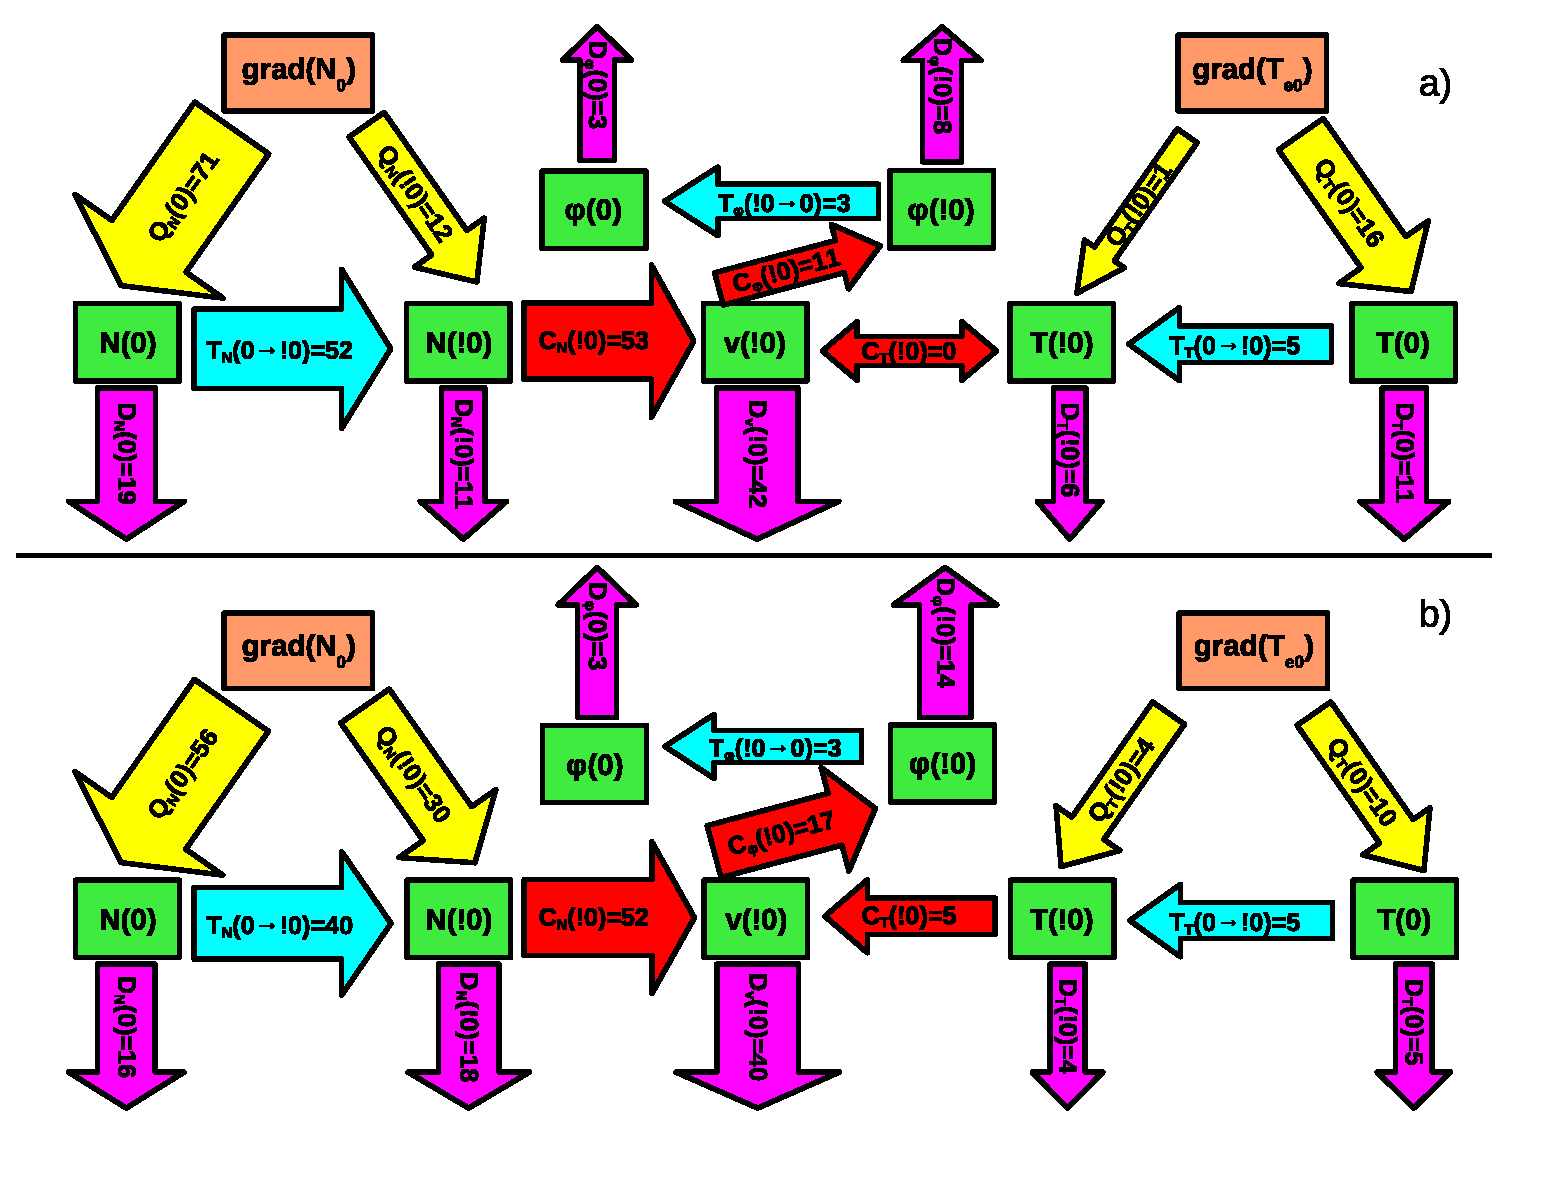
\includegraphics[width=0.9\textwidth]{energy_diagrams}
\hfil
\caption{Summary of the energy dynamics for the \textbf{a)} periodic case and \textbf{b)} sheath boundary case. Each arrow contains the sum over all $m$. The 0's in the parentheses
represent the $n=0$ modes while the !0's represent a sum over the $n$ modes for $n \ne 0$. The values in the arrows represent the percentage of total energy that goes through the channel
represented by the arrow. The size of the arrows gives a rougher but more visual indication of the amount of energy going through each channel.}
\label{en_diagrams}
\end{figure}

The diagrams in Fig.~\ref{en_diagrams} summarize the flow of energy for the periodic and sheath simulations. Each of the functions, such as $Q_n(m,n)$, is a function of $m$ and $n$, making
visualization of all of these functions difficult. So the terms in the diagrams are summed over $m$. Additionally, all of the $n \ne 0$ terms are summed over as well.
The $n=0$ contribution is separated from the other $n$ components because
the $n=0 \leftrightarrow n \ne 0$ dynamic is the primary factor that determines whether the linear instability or the nonlinear instability dominates the energy drive~\cite{friedman2012b}.

In these diagrams, the source of energy into the fluctuations is free energy in the equilibrium gradients, $\nabla N_0$ and $\nabla T_{e0}$. The arrows labeled $Q_n$ and $Q_t$ represent energy injection from
the equilibrium gradients into the fluctuations, $n(\vec{k})$ and $t(\vec{k})$, the only net deposition of energy into the fluctuations. A majority of the energy deposited into the fluctuations ($71\%$
for the periodic simulation and $56\%$ for the sheath simulation)
is from the density gradient into the $n=0$ density fluctuations. This is not a path allowed by any of the linear instabilities in the system since
the linear instabilities can only deposit energy into $n \ne 0$ fluctuations.
In fact, in this turbulent state, more energy is transfered by nonlinear three-wave coupling into $n \ne 0$ fluctuations than by direct injection from the equilibrium gradients. The three wave
coupling is represented by the $T_n$ and $T_t$ arrows. The direction of these arrows is from $n=0 \rightarrow n \ne 0$, which is in opposition to the common cascading type 
turbulent paradigm where the linear instability dominates the turbulent injection dynamics and three-wave processes transfer energy to waves that are linearly stable.

Now, the reason why all of the non-dissipated energy that is injected into $n=0$ density and temperature structures goes into $n \ne 0$ density and temperature potential energy structures rather than into $n=0$
kinetic energy structures is that potential to kinetic energy transfer can only occur through the adiabatic response, which requires finite $n$. Actually, in the sheath simulation, potential energy
can transfer to kinetic energy through the axial boundaries, but this still requires finite $n$ and it works only through the temperature fluctuations, which are less important than the density
fluctuations in the simulations. So the main transfer channel from potential to kinetic energy, shown by the $C_n$, $C_t$, and $C_\phi$ arrows, is the adiabatic response. The adiabatic response takes energy
from the $n \ne 0$ density and temperature fluctuations and transfers it into the parallel velocity fluctuations ($C_n$ and $C_t$, respectively). It then transfers some of this energy into
$n \ne 0$ potential fluctuations ($C_\phi$), while much of the fluctuation energy is ohmically dissipated ($D_v$).

The final step of the energy dynamics process is a three-wave axial wavenumber transfer from potential fluctuations at $n \ne 0$ to potential fluctuations at $n=0$, which is a neccessary component
in driving the $Q_n(0)$ and $Q_t(0)$ injections. Meanwhile, dissipation acts on all fluctuations, which is quantified by the $D$ arrows throughout. A couple of interesting features are evident
from the diagrams in Fig.~\ref{en_diagrams}. First, the turbulent dynamics in both simulations are dominated by the nonlinear instability process described above and in Friedman et al.~\cite{friedman2012}
rather than the paradigmatic process of linear instability energy injection followed by nonlinear cascading. And second,
the periodic and sheath simulations have qualitatively similar dynamics despite the fact that the linear stability properties of the two cases
are qualitatively different. This speaks to the robustness of the nonlinear instability.

A more compact way to see the similarity of the instability process in the periodic and sheath simulations is shown in Fig.~\ref{nl_vs_lin_gamma}. 
This figure shows the turbulent growth rate of the two simulations along with that of the no $n=0$ simulation, which really contrasts the periodic and sheath simulations. 
The turbulent growth rate is defined as the net energy injection
into the fluctuations minus the dissipation out of them, all divided by the total energy. The conservative transfers are of course not part of the growth rates.
Formally, $\gamma(\vec{k}) = (\sum_j Q_j(\vec{k}) + D_j(\vec{k}))/E_{tot}(\vec{k})$, where the index j represents the different fields.
Since the growth rates sum over the fields, it's not as difficult to view them in their full wavenumber space (both in $m$ and $n$). However, almost all of the energy in the simulations is 
contained in $n=0$ and $n=1$ fluctuations, so $n>1$ fluctuations are not shown in the figure. It should be noted, however, that Fourier decomposing the sheath simulation in the axial direction
is less ideal than doing so in the periodic simulation. Fourier modes are not as natural a basis in the sheath simulation, and the $n=1$ Fourier mode does not perfectly represent the linear
eigenmode structure as it does for the periodic and no $n=0$ simulations. 
A more detailed discussion of this point is left to the Appendix, but in summary, the $n=1$ Fourier mode does capture enough of the sheath
linear eigenmode structure to make the Fourier decomposition useful for this simulation.

Figure~\ref{nl_vs_lin_gamma} illustrates the true dominance of the nonlinear instability in the positive $n=0$ energy growth rate and negative $n=1$ growth rate for the periodic and sheath simulations. 
It also reveals the remarkable similarity in the nonlinear energy dynamics processes between the periodic and sheath simulations. This is in stark contrast to the no $n=0$ simulation, which has an $n=1$
growth rate similar to the linear growth rate (Fig.~\ref{drift_cwm_gamma}) and a negative $n=0$ growth rate. Note that even though the $n=0$ fluctuation components are removed from this simulation at each time
step, $n=0$ fluctuations are nonlinearly excited (by three-wave transfer) by the $n \ne 0$ fluctuations, and therefore, they do have small but finite amplitude prior to their removal, which can be used to
calculate the growth rate of these modes. Furthermore, the turbulent growth rate of the $n=1$ component of the no $n=0$ simulation is
slightly less than the linear growth rate for all $m$ due to the fact that eigenmodes other than the fastest growing ones are nonlinearly excited in the turbulent simulation, thus damping the growth rate.
This no $n=0$ growth rate picture is just that of the turbulence paradigm of linear instability with cascading dynamics. Again, this is much different than the picture of the periodic and sheath simulations
which are dominated by a nonlinear instability process, in which the $n=0$ and $n=1$ growth rates have the opposite sign of the linear growth rates.


\begin{figure}[!htbp]
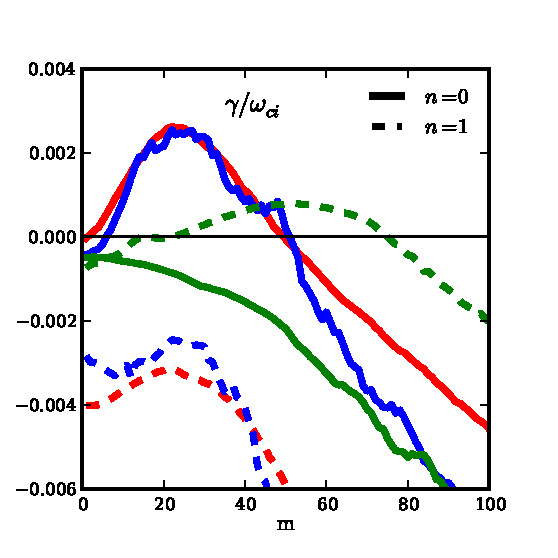
\includegraphics[]{lin_vs_nl_gamma}
\hfil
\caption{ The turbulent growth rates defined as $\pdiff{E_{tot}}{t}/(2 E_{tot})$ where only the linear terms are included in $\pdiff{E_{tot}}{t}$. The $n=0$ (solid) and $n \ne 0$ (dashed) 
contributions are separated.}
\label{nl_vs_lin_gamma}
\end{figure}



\section{Linear vs Nonlinear Structure Correlation}
\label{Sec_lin_vs_nl}
\subsection{Energy in the Fastest Growing Eigenmodes}
\label{subsec_en_eigenmodes}

Now it may be the case that in simulations dominated by a linear instability, the fastest growing linear
eigenmode dominates the system, nonlinearly transfering some energy to more weakly unstable or even stable eigenmodes. In this case, a large portion of the energy may remain in the fastest
growing linear eigenmode~\cite{hatch2011}. In the case where a nonlinear instability is dominant, the linear eigenmode should have little bearing on the structure of the turbulence and therefore little
energy should be contained in this eigenmode. Therefore, a guage of whether a linear or nonlinear instability dominates a system is the fraction of energy in a turbulent system
that is contained in the fastest growing linear eigenmode. This may be calculated by projecting the fastest growing eigenmode onto the turbulent state.

Formally, in the model considered in this study, the turbulent state is fully described by four independent fields, which can be appended into a single vector of the spatio-temporal field functions: 
$f_{turb}(\vec{r},t) = (N(\vec{r},t),T_e(\vec{r},t),\gradperp \phi(\vec{r},t), \vpe(\vec{r},t))$. This vector may be decomposed in a complete basis:

\beq
\label{basis_decomp}
f_{turb}(\vec{r},t) = \sum_{i,m} c_{i,m}(t) v_{i,m}(r,z) e^{i m \theta},
\eeq

where $v_{i,m}(r,z)$ are time-independent spatial complex basis functions (of the form $v_{i,m}(r,z) = \left\{ n_{i,m}(r,z),t_{i,m}(r,z),\gradperp \phi_{i,m}(r,z), v_{i,m}(r,z) \right\}$)
and $c_{i,m}(t)$ are the complex time-dependent amplitudes. The $\theta$ dependence of the basis functions has been explicitly imposed as a Fourier basis. The total number of
linearly independent basis functions is the number of total grid points used in the simulation times the number of independent fields, which is four in this case.
Now, $v_{i,m}(r,z)$ can be any linearly independent set of functions and need not be the linear eigenfunctions
of the system. In fact, the linear eigenfunctions of the equations used here are not orthogonal, and are thus not very useful to consider. However, it is quite useful to set $v_{0,m}(r,z)$ to the fastest
growing linear eigenmode because this is the structure of interest that is to be projected onto the turbulence. 
The other $v_{i \ne 0,m}(r,z)$ comprise the remainder of the orthonormal basis, and they must be different from
the remaining linear eigenfunctions in order to complete the orthogonal basis. It isn't necessary for the purpose of this study to actually compute these other basis functions, but if one were to compute
them, one might start with all of the linear eigenmodes
and perform a Gram-Schmidt orthogonalization procedure, starting with the fastest growing mode and orthogonalizing the others. Using this procedure, Hatch et al.~\cite{hatch2011}
found that a significant fraction (number?) of the energy in a turbulent state of ITG turbulence was contained in the fastest growing linear eigenmode at each perpendicular wavenumber.
Such a result, however, doesn't require knowledge of the other basis functions, and thus they are not computed here.

Now, to compute this fraction, first define an inner product that is energetically meaningful and that sets the orthonormality of the basis functions:

\beq
\label{basis_orthonormality}
\left< v_{i,m},v_{j,m} \right> = \int w v_{i,m}^* \cdot v_{j,m} dV = \delta_{i,j}.
\eeq

The weighting $w$ is such that $\left< f_{turb}, f_{turb} \right> = E_{turb}$.
Now from Eqs.~\ref{basis_decomp} and~\ref{basis_orthonormality}, $\left< f_{turb}, f_{turb} \right> = E_{turb} = \sum_{i,m} |c_{i,m}|^2$ and 
$\left< f_{turb,m}, f_{turb,m} \right> = E_{turb,m} = \sum_i |c_{i,m}|^2$.
Now, the amount of energy contained in the fastest growing mode (for each $m$) is given by the square of the projection
of the mode onto the turbulence: $E_{0,m} = \left| \left< v_{0,m}, f_{turb,m} \right> \right|^2 = |c_{0,m}|^2$. The ratio 
$R_m = E_{0,m}/E_{turb,m}$ is a measure of the fraction of turbulent energy contained in the fastest growing linear eigenmode. 

Of course, $E_{turb,m}$ is easily calculated from the turbulent state, but $E_{0,m}$ in the 
turbulent state can only be found with knowledge of the fastest growing eigenfunction. The fastest growing eigenfunctions, though, can be found easily by running a simulation from a random 
or turbulent state with all of the nonlinearities removed from the model equations as was done in Section~\ref{sec_linear}. After some time, the fastest growing eigenfunctions will come to
dominate the fluctuation structure. Then, a Fourier decomposition in $m$ space will separate the fastest growing eigenfunctions at each $m$, including the real and imaginary part
of the eigenfunctions (up to a time dependent complex constant, which is removed by normalizing the eigenfunction). These eigenfunctions can then be projected onto the turbulent state
with the inner product defined in Eq.~\ref{basis_orthonormality}.

The ratio $R_m$ is shown in Fig.~\ref{ratios} for the three simulations.


\begin{figure}[!htbp]
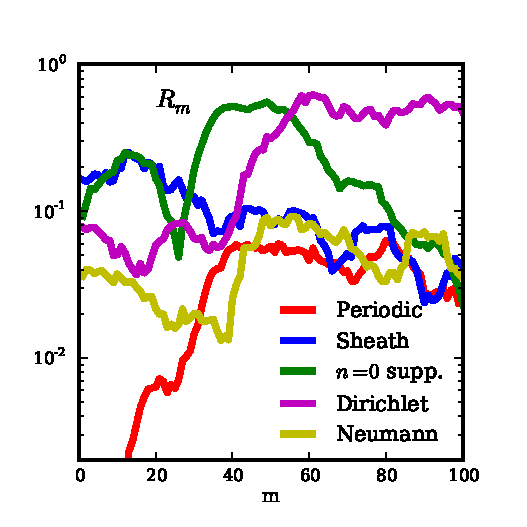
\includegraphics[]{ratios}
\hfil
\caption{$R_m$ for all $m$ for the periodic, sheath, and no $n=0$ simulations.}
\label{ratios}
\end{figure}


\subsection{Quasilinear Flux}
\label{subsec_quasilinear}

Another consequency of the linear instability being overshadowed by the nonlinear instability in the turbulent state is that calculations of turbulent characteristics that rely upon linear properties may be
highly inaccurate. An obvious contender for such a calculation is the quasilinear flux.
The electrostatic radial particle flux on a given flux surface is

\beq
\label{rad_flux}
\Gamma(r) = \int n v_r dS = \int - \sum_m i m n_m \phi_m^* dz.
\eeq

The flux in the turbulent state depends upon the correlation of two independent quantities, however, a widely used method for evaluating the correlation between the density and potential is
to use a linear eigenvector to express $n_m$ in terms of the potential: $n_m = L(m) \phi_m$, where $L(m)$ is the linear response function~\cite{terry2006a}. 
Substitution of this expression into Eq.~\ref{rad_flux} yields the quasilinear flux:

\beq
\label{ql_flux}
\Gamma_{QL}(r,m) = \int - i m |\phi_m|^2 L(m) dz.
\eeq

The potential amplitude $|\phi_m|^2$ is obtained from the turbulent state, but the linear response function must be obtained from the linear eigenvectors, typically the fastest growing
linear eigenvectors. The full nonlinear flux and the quasilinear flux are shown for the three simulations in Fig.~\ref{flux_comparison}.

\begin{figure}[!htbp]
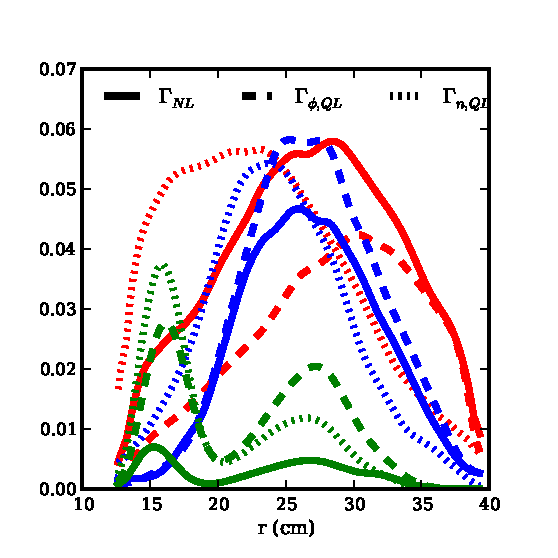
\includegraphics[]{flux_comparison}
\hfil
\caption{The radial particle flux calculated from the turbulence vs. the corresponding quasilinear flux.}
\label{flux_comparison}
\end{figure}


\section{Conclusion}

\begin{acknowledgments}
This research was performed under appointment to the Fusion Energy Sciences Fellowship Program administered by Oak Ridge Institute for
Science and Education under a contract between the U.S. Department of Energy and the Oak Ridge Associated Universities. 
\end{acknowledgments}


\appendix


\section{Non-periodic Fourier Decomposition}

\begin{figure}[!htbp]
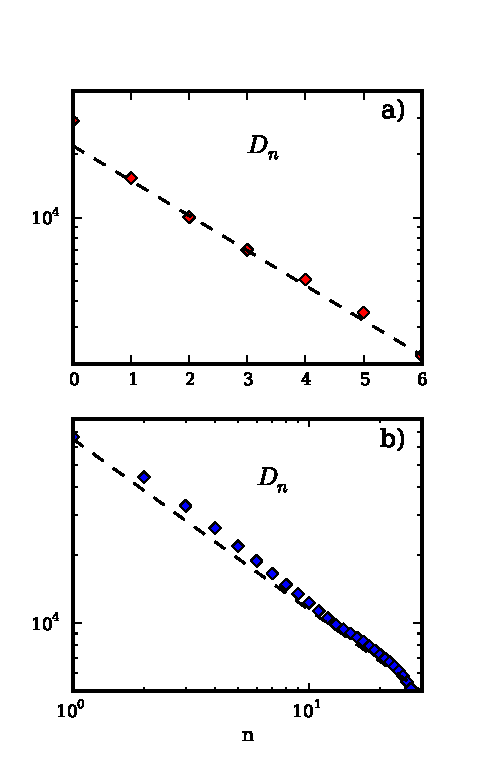
\includegraphics[]{fourier_convergence}
\hfil
\caption{$D_n$ for \textbf{a)} The simulation with periodic axial
boundaries displaying exponential convergence and \textbf{b)} the simulation with sheath axial boundaries displaying algebraic convergence.}
\label{fourier_convergence}
\end{figure}

It is well known that Fourier reconstructions of signals that contain discontinuities or non-periodic boundaries are subject to Gibbs phenomena. A clear indication of this is the
convergence properties of the Fourier reconstructions. Take a discrete signal with the following Fourier decomposition:

\beq
\label{f_decomp}
f(x) = \sum_{k=-N}^{N} \hat{f}_k e^{2 \pi i k x},
\eeq

where the $\hat{f}_k$ are ordered in the sum by the size of their absolute value with $\hat{f}_0$ being the largest Fourier coefficient. The Fourier reconstruction of order $n<N$ is then:

\beq
\label{f_recon}
g_n(x) = \sum_{k=-n}^{n} \hat{f}_k e^{2 \pi i k x}
\eeq

There are several types of convergences of the $g_n$, one of which is the $L1$ norm. Defining the difference between the original signal and the Fourier reconstruction of order $n$ as
$D_n = \sum_x |f(x) - g_n(x)|$, one can look at the convergence of $D_n$ as a function of $n$. For periodic signals, $D_n$ converges exponentially, while it only converges algebraically
(power law) for non-periodic or discontinuous signals. $D_n$ is plotted for the cases of the two simulations
(one with periodic axial boundary conditions and the other with sheath boundary conditions) in Fig.~\ref{fourier_convergence}.





\bibliography{refs}
\bibliographystyle{unsrt}

\end{document}
